\chapter{Experiments} \label{chapter:experiments}

In this chapter, we evaluate how effective our learned cost function is, which is described below, where $D$ is the number of features, $A$ is the set of actions and the resulting value of $\mathbf{x}$ after the interventions is $\mathbf{x}^{\text{PCF}}$.

\begin{align} \label{eq:cost_function_experiments}
	\cost(A, \beta_k, \mathcal{F}) & = \sum_{i=1}^D \delta_i \beta_{ki}^2 \\ \nonumber
	A & = \big\{(\mathbf{S}, \text{do} \{\mathbf{x}_i:=\mathbf{x}_i + \boldsymbol{\delta}_i\}_{i=1, \ldots, D})\big\} \\ \nonumber
	\mathbf{x}^{\text{PCF}} & = \mathbb{I}_{i \in I} \boldsymbol{\delta}_i + \bigg( \mathbf{x}_i + f_i(\textbf{pa}^{\text{PCFF}}_i) - f_i(\textbf{pa}_i) \bigg)
\end{align}

\section{End-to-End Methodology}

The end to end methodology for generating recourse with a learned cost is shown in Figure \ref{fig:workflow}, and more details on each of the steps in the methodology are described below.

\begin{figure}[!htb]
	\centering
	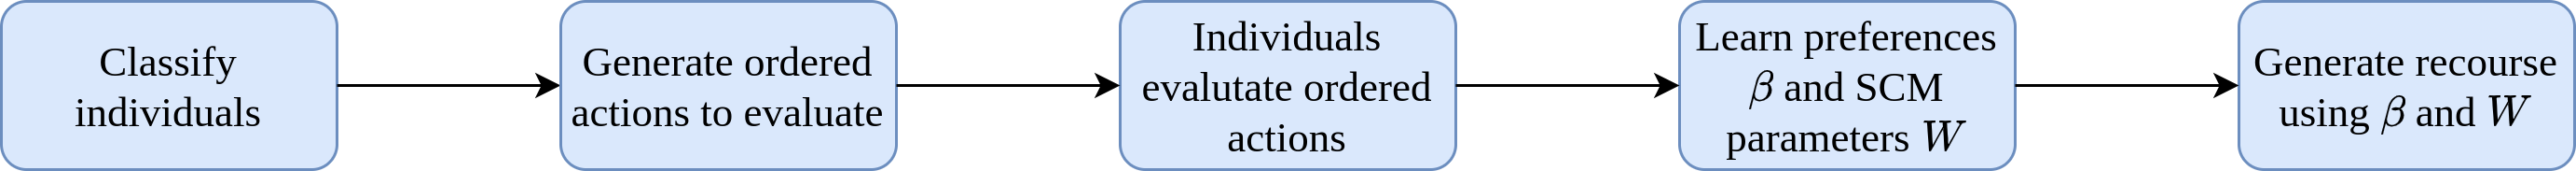
\includegraphics[width=\linewidth]{images/draw.io/workflow.png}
	\caption{End-to-End Methodology}
	\label{fig:workflow}
\end{figure}

\begin{enumerate}
	\item \textbf{Classify individuals}. Individuals with features $\mathbf{X}$ are assessed by a classifier and are classified either positively (e.g., loan approved, admission acceptance) or negatively (e.g., loan rejected, admission rejected). In this thesis, logistic regression has been used, largely for simplicity. However, as an augmented Lagrangian gradient descent optimisation is used to generate recourse (see section \ref{section:generating_recourse}), any differentiable classifier could be used instead of logistic regression.
	
	\item \textbf{Generate ordered actions to evaluate}. We randomly generate actions for each negatively classified individual and associated randomly generated orderings. This is another area for future work, where an online or Bayesian approach could be used to generate recourse actions in order to maximise information gain, such as the approach used in \textcite{detoniPersonalizedAlgorithmicRecourse2023}.
	
	\item \textbf{Users evaluate ordered actions}. Using the cost function described in equation \ref{eq:cost_function_experiments} with noisy user preferences $\tilde{\beta_k}$ and noisy SCM $\tilde{\mathcal{F}}$, users evaluate which of the ordered actions they are presented with they prefer. 
	
	\item \textbf{Learn preferences $\hat{\beta_k}$ and SCM approximation parameters $\hat{W}$}. The model deployer then learns user preferences $\hat{\beta_k}$ and a linear approximation of the true SCM $\hat{W}$ using the optimisation presented in section \ref{section:cost_learning_formulation}.
	
	\item \textbf{Generate recourse using $\hat{\beta_k}$ and $\hat{W}$}. The model deployer then generates recourse $\mathbf{X}^*$ for the negatively classified users.
	
\end{enumerate}



\section{Synthetic Data}

We create synthetic SCMs from which we sample our 

\begin{align}
	x_1 & = u_1 & u_1 \sim N(0,1) \\ \nonumber
	x_2 & = 0.5x_1 + u_2 & u_2 \sim N(0,1) \\ \nonumber
	x_3 & = 0.2x_1 + 0.3x_2 + u_3 & u_3 \sim N(0,0.5) \\ \nonumber
	y   & \sim \text{Bernoulli}(\sigma(0.1x_1 + 0.2x_2 + 0.3x_3))
\end{align}

Ground truth $\beta$: [0.5, 0.333, 0.1667]


\begin{figure}[!htb]
	\centering
	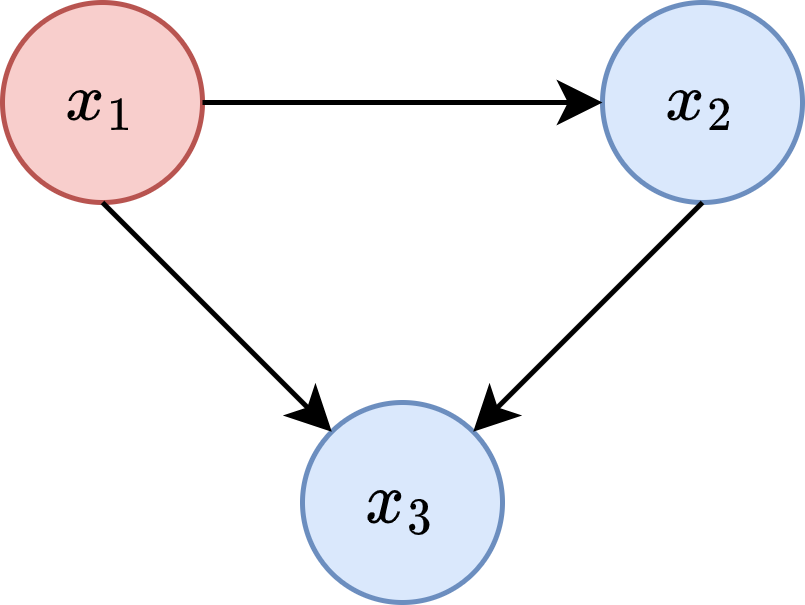
\includegraphics[width=0.4\linewidth]{images/draw.io/toy_scm.png}
	\caption{Simple SCM}
	\label{fig:simple_scm}
\end{figure}


\subsection{Noiseless responses with perfect knowledge of the causal graph}

Ground truth $\beta$: [0.5, 0.333, 0.1667] \\
Learned $\beta$ : [0.4965, 0.3355, 0.1681]

\subsection{Noiseless responses with imperfect knowledge of the causal graph}

Ground truth $\beta$: [0.5, 0.333, 0.1667] \\
Learned $\beta$ : [0.4975, 0.3354, 0.1671]

Ground truth $W$: $\begin{bmatrix}
	0 & 0.5 & 0.2 \\
	0 & 0 & 0.3 \\
	0 & 0 & 0
\end{bmatrix}$

Learned $W$: $\begin{bmatrix}
	0 & 0.4864 & 0.2136 \\
	0.0033 & 0 & 0.3221 \\
	0.0008 & 0.0086 & 0
\end{bmatrix}$


\subsection{Noisy responses}

So far, only noisy responses have been added (not noise knowledge of the causal graph)

\textbf{With noise distribution $N(0, 0.1)$:}

Ground truth $\beta$: [0.5, 0.333, 0.1667] \\
Learned $\beta$ : [0.4917, 0.3418, 0.1665]

Ground truth $W$: $\begin{bmatrix}
	0 & 0.5 & 0.2 \\
	0 & 0 & 0.3 \\
	0 & 0 & 0
\end{bmatrix}$

Learned $W$: $\begin{bmatrix}
	0 & 0.5424 & 0.1683 \\
	-0.0070 & 0 & 0.3950 \\
	0.0166 & -0.0007 & 0
\end{bmatrix}$


\textbf{With noise distribution $N(0, 0.5)$:}

Ground truth $\beta$: [0.5, 0.333, 0.1667] \\
Learned $\beta$ : [0.4224, 0.3686, 0.2090]

Ground truth $W$: $\begin{bmatrix}
	0 & 0.5 & 0.2 \\
	0 & 0 & 0.3 \\
	0 & 0 & 0
\end{bmatrix}$

Learned $W$: $\begin{bmatrix}
	0 & 0.5772 & 0.3522 \\
	-0.0062 & 0 & 0.1657 \\
	0.0974 & 0.0459 & 0
\end{bmatrix}$

\textbf{With noise distribution $N(0, 2)$:}

Ground truth $\beta$: [0.5, 0.333, 0.1667] \\
Learned $\beta$ : [0.4958, 0.2685, 0.2357]

Ground truth $W$: $\begin{bmatrix}
	0 & 0.5 & 0.2 \\
	0 & 0 & 0.3 \\
	0 & 0 & 0
\end{bmatrix}$

Learned $W$: $\begin{bmatrix}
	0 & 0.5353 & 0.08712 \\
	-0.1487 & 0 & 0.7206 \\
	-0.2152 & 0.2409 & 0
\end{bmatrix}$